\chapter[Análise dos Resultados]{Análise dos Resultados}

\section{Fase 1: Análise e Preparação de Dados}
\subsection{OE1 - Expansão, Processamento e Análise de Dados para Predição de Ploidia}
\subsubsection{Atividade 1 (A1): Análise, Revisão, Seleção e Limpeza de Variáveis para Predição de Euploidia}
Na fase inicial da tarefa (A1), realizamos uma análise, revisão e escolha das variáveis para o nosso modelo de IA. Através do estudo bibliográfico, conseguimos verificar um grupo de variáveis da planilha de dados que possui fundamentação científica que evidenciam sua importância para a evolução do modelo. As variáveis selecionadas para o nosso estudo serão: \textbf{Idade, t2, t3, t4, t5, t8, s2, cc2, tSC, tSB, tB, cc3 (t5-t3), s3 (t8-t5), t5-t2, tSC-t8, tB-tSB, Estágio, Morfo e KIDScore}. 

A coluna de \textbf{Plodia} também foi selecionada, pois nos possibilita agrupar os embriões em duas categorias claras, distinguindo entre aqueles com euploidia normal e aqueles com alterações cromossômicas, o que é crucial para a elaboração de um modelo sólido.

Não identificamos estudos que estabelecem uma ligação direta entre o parâmetro \textbf{st2} e a previsão de euploidia. Apesar do movimento citoplasmático antes da citocinese ser um marco significativo no desenvolvimento embrionário, a ausência de provas científicas que liguem esse movimento à qualidade do embrião e à euploidia nos levou a remover o \textbf{st2} da lista de variáveis para o modelo. Igualmente, não foram identificados estudos que analisassem especificamente o intervalo entre \textbf{t2} (o instante em que o embrião alcança a fase de duas células) e \textbf{st2} (movimento citoplasmático pré-citocinese) para prever a euploidia. Como \textbf{st2} foi eliminada, também removemos o parâmetro \textbf{t2-st2} do nosso grupo de variáveis

A partir do estudo bibliográfico minucioso realizado na seção de \textbf{Atividade 1 do Capítulo 4}, conseguimos determinar quais variáveis são fundamentais para a elaboração do nosso modelo de previsão de euploidia. Depois de examinar e revisar as variáveis, modificamos a planilha para espelhar os dados mais significativos para o modelo, que se encontra no Anexo \ref{anexo:planilha-revisada} como \textbf{"Planilha Revisada - Colunas Excluídas"}. Portanto, as colunas \textbf{Id, Data da biópsia e Embrião n.} foram eliminadas, uma vez que não contribuem para o valor do modelo. Adicionalmente, as variáveis \textbf{st2} e \textbf{t2-st2} foram eliminadas, conforme mencionado anteriormente. Portanto, a planilha revisada agora inclui somente as variáveis que possuem uma ligação comprovada com a previsão de euploidia, fundamentada nas evidências científicas revisadas.

Ao tratar de \textbf{dados ausentes} em conjuntos de dados, utilizando o método Análise de Casos Completos (ACC), possuíamos 84 linhas de dados, das quais apenas 2 têm dados ausentes. Na \textbf{"Planilha com Indicação de Dados Ausentes"} (Anexo \ref{anexo:planilha-dados-ausentes}), os campos que não possuem dados estão em preto. Por esse motivo, excluímos essas duas linhas de modo manual, já que é um número muito pequeno para fazer um código de limpeza de dados, assim, a planilha se modifica se tornando a \textbf{"Planilha de Dados Refinados"} presente no Anexo \ref{anexo:planilha-refinada}, resultando em 82 linhas, que está nos anexos. 

\subsubsection{Atividade 2 (A2): Identificação da Correlação entre os Parâmetros na Previsão da Ploidia do Embrião}

A análise de correlação foi realizada com o objetivo de identificar as interações mais significativas entre os parâmetros relacionados ao desenvolvimento embrionário e a ploidia. Para isso, foi utilizado o coeficiente de Spearman, explicado no \textbf{APÊNDICE \ref{apendice:spearman}}. A análise das relações entre as variáveis possibilitou a identificação das variáveis que se afetam e afetam a porcentagem de euploidia, fornecendo um alicerce para a melhoria de processos e tomada de decisões da IA. A consolidação dos resultados resultou em dois documentos: um arquivo Excel (\textit{correlation\_results.xlsx}) que apresenta uma visão aprofundada dos coeficientes calculados, transformado em um PDF mais compacto para facilitar a visualização, disponível nos anexos, e um documento Word (\textit{relatorio\_correlacoes.docx}) que contém todos os gráficos de dispersão para as combinações examinadas e valores de correlação relacionados, totalizando 172 páginas. Caso haja interesse em consultar o documento completo, siga os passos descritos na “Atividade 2” no GitHub do projeto: \textit{GitHub-TCC}. Executando o código, é possível gerar o documento completo.

\subsection*{correlation\_results}

A função \texttt{spearman} da biblioteca \texttt{SciPy} foi empregada para gerar o coeficiente de Spearman no código, calculando tanto o coeficiente de correlação quanto o valor-p para cada par de variáveis. Inicialmente, o código importou as informações do arquivo \textit{"Planilha de Dados Refinados"} presente no Anexo \ref{anexo:planilha-refinada}, reconheceu as colunas numéricas pertinentes e iterou sobre todas as combinações possíveis de variáveis, assegurando que uma variável não fosse comparada a si mesma.

Os resultados gerados na planilha \textit{correlation\_results} incluem três colunas:
\begin{itemize}
    \item \textbf{Variable 1:} A primeira variável da análise.
    \item \textbf{Variable 2:} A segunda variável correlacionada.
    \item \textbf{Spearman Coefficient:} O coeficiente calculado para o par de variáveis.
\end{itemize}

Os coeficientes de correlação de Spearman, foram calculados a partir de todas as combinações possíveis de variáveis escolhidas da base de dados, que está presente de forma mais enxuta nos anexos. Cada linha identifica um par de variáveis examinadas, com os seus resultados apontando a intensidade e a direção (positiva ou negativa) da correlação entre elas. Ressaltando que, uma correlação positiva perfeita é representada por um valor de +1 que indica que o crescimento de uma variável está sempre ligado ao crescimento da outra. Por outro lado, um valor de -1 indica uma correlação negativa perfeita, em que o aumento de uma variável corresponde consistentemente à diminuição da outra. Quando o coeficiente é zero, indica que as variáveis não possuem uma relação monotônica evidente, isto é, não existe um padrão consistente de variação conjunta. 

\subsection*{relatorio\_correlacoes}

O documento \textit{relatorio\_correlacoes.docx} foi gerado automaticamente usando a biblioteca \texttt{python-docx}, que permite a criação e manipulação de documentos Word. Depois de obter os coeficientes de Spearman para cada par de variáveis como descrito e apresentado no documento \textit{“correlation\_results”} explicado acima, o código itera sobre essas combinações. 

Este documento fornece uma avaliação minuciosa das correlações, com os gráficos de dispersão para cada par de variáveis e os valores dos coeficientes de Spearman, em que esses valores estão escritos com seu sinal de positivo ou negativo, seguido de duas casas decimais. O documento é necessário para entender padrões particulares e enfatizar relações relevantes de forma visual.

Em seguida, apresentaremos a avaliação dos resultados mais relevantes obtidos a partir dos dois documentos produzidos pelo código, ressaltando as variáveis que possuem ligações mais sólidas entre si, assim como as que possuem pouca ou nenhuma interação recíproca. Esses resultados serão comparados com as referências bibliográficas anteriormente discutidas.


\subsection*{Idade}

Nos gráficos seguintes, a variável \textit{Idade} está representada pelo marcador “o” em verde claro, enquanto as demais variáveis estão identificadas com o marcador “x” em azul escuro. 

A correlação com \textbf{t4} (-0,15) na Figura \ref{fig:idade-t4} sugere que a idade exerce uma influência leve sobre eventos específicos do desenvolvimento embrionário. Mulheres mais velhas podem apresentar embriões com ligeiro atraso no tempo necessário para atingir o estágio \textit{t4}. Embora a influência da idade no ritmo inicial de desenvolvimento seja limitada, há uma leve tendência de atraso.

\begin{figure}[h]
    \captionsetup{font=footnotesize, justification=centering, labelsep=period, position=above}
    \caption{Dispersão entre Idade e t4 - Coeficiente de Spearman: -0,15}
    \label{fig:idade-t4}
    \centering
    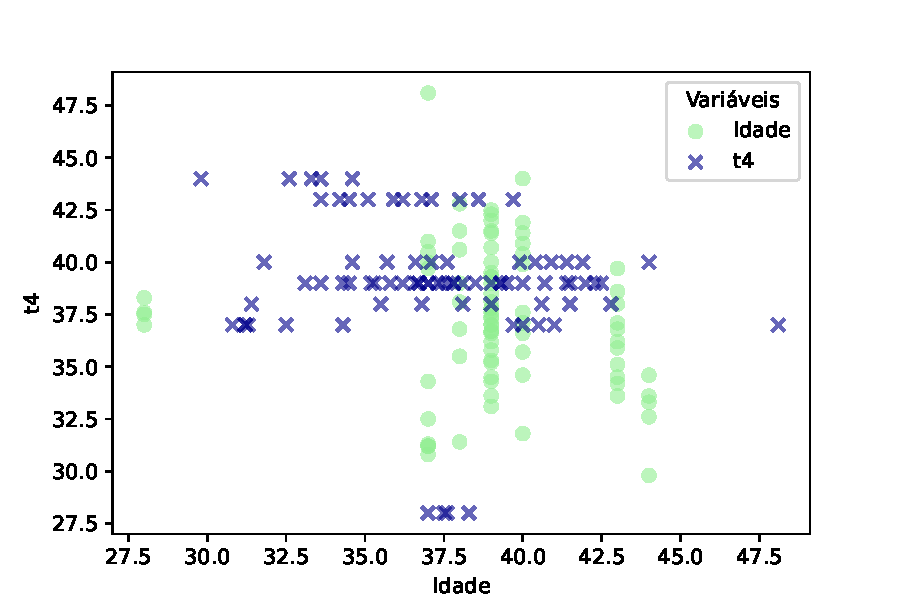
\includegraphics[scale=0.3]{figuras/Spearman/idade-t4.pdf}
    \vspace{0.3cm} 
    \begin{minipage}{\linewidth}
        \centering
        \scriptsize{Fonte: Autoras (2025)}
    \end{minipage}
\end{figure}
\FloatBarrier

Em relação ao tempo para 5 células, \textbf{t5} (0.11), obteve uma correlação positiva. Isso sugere uma tendência muito sutil de que embriões em fases mais avançadas estejam ligados a mães de mais idade, como observado na Figura \ref{fig:idade-t5}.

\begin{figure}[h]
    \captionsetup{font=footnotesize, justification=centering, labelsep=period, position=above}
    \caption{Dispersão entre Idade e t5 - Coeficiente de Spearman: 0,11}
    \label{fig:idade-t5}
    \centering
    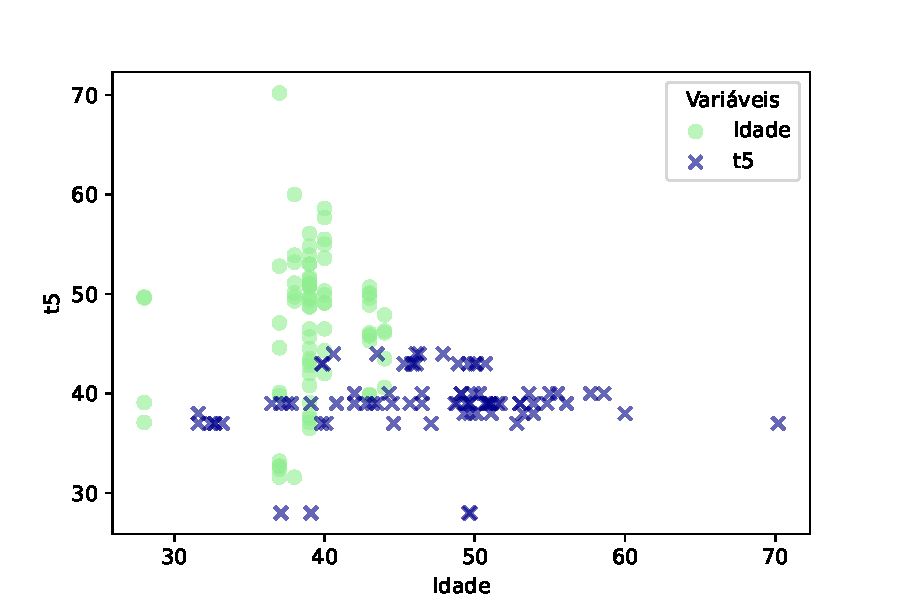
\includegraphics[scale=0.3]{figuras/Spearman/idade-t5.pdf}
    \vspace{0.3cm} 
    \begin{minipage}{\linewidth}
        \centering
        \scriptsize{Fonte: Autoras (2025)}
    \end{minipage}
\end{figure}
\FloatBarrier

Ao reparar em alguns índices negativos, observamos os índices \textbf{tSB (-0.10), cc2 (t3-t2) (-0.17), s2 (t4-t3) (-0.24),  s3 (t8-t5) (-0.28) e a Ploidia(-0.50)}. Nota-se que os coeficientes mais próximos de 0 (como -0,10 a -0,28) indicam uma correlação negativa fraca. Isso traduz que há uma tendência muito sutil de que, quando uma variável aumenta, a idade, a outra diminui. Em \textbf{tSB} Figura \ref{fig:idade-tSB}, o coeficiente negativo insinua que o tempo de formação inicial da blastocisto tende a ser menor em embriões provenientes de mães mais velhas. Na variável \textbf{cc2}, Figura \ref{fig:idade-cc2}, a correlação desfavorável sugere uma maior irregularidade no intervalo entre a segunda e a terceira divisão celular (t2 para t3) em embriões de mães mais velhas. Em \textbf{s2} (Figura \ref{fig:idade-s2}) e \textbf{s3} (Figura \ref{fig:idade-s3}), mostra que a idade materna também está ligada a uma diminuição na eficácia do intervalo entre as divisões celulares de t3 para t4. Isso indica um efeito na fase intermediária do ciclo celular. Nos embriões de mães mais velhas, o período entre a fase de 8 células e a formação do blastocisto final é estendido, sinalizando obstáculos no progresso dessas fases. Todos esses atrasos podem ser cruciais, já que fases iniciais bem sincronizadas são fundamentais para um desenvolvimento embrionário adequado, mostrando como uma idade avançada pode afetar o desenvolvimento embrionário, afirmando a bibliografia estudada, fato já citado por \citeonline{borges2019}, que reitera que a idade materna exerce maior influência sobre a qualidade embrionária.

\begin{figure}[h]
    \captionsetup{font=footnotesize, justification=centering, labelsep=period, position=above}
    \centering
    \begin{minipage}[b]{0.45\linewidth}
        \caption{Dispersão entre Idade e tSB Coeficiente de Spearman: -0.10}
        \label{fig:idade-tSB}
        \centering
        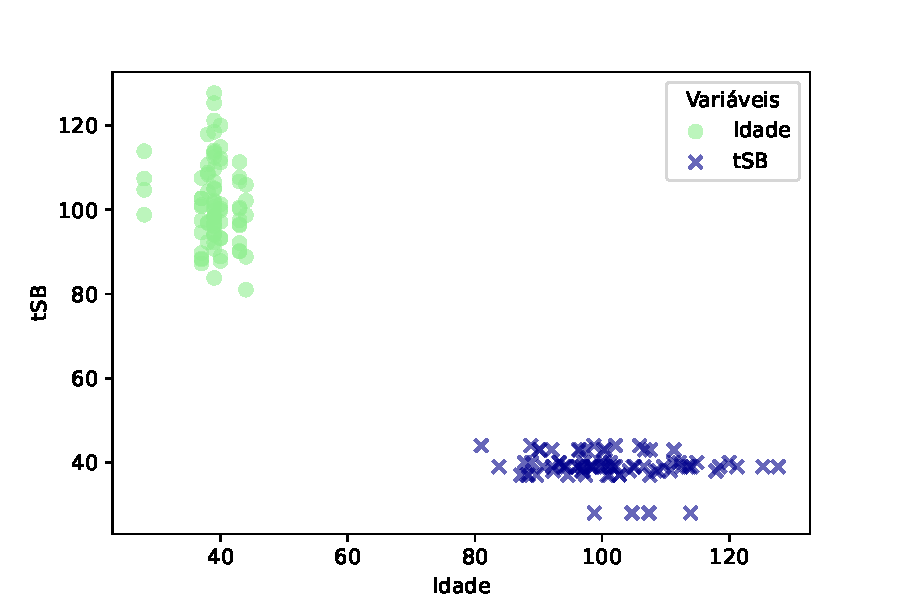
\includegraphics[scale=0.47]{figuras/Spearman/idade-tSB.pdf}
        \vspace{0.3cm}
        \begin{minipage}{\linewidth}
            \centering
            \scriptsize{Fonte: Autoras (2025)}
        \end{minipage}
    \end{minipage}
    \hspace{0.05\linewidth}
    \begin{minipage}[b]{0.45\linewidth}
        \caption{Dispersão entre Idade e cc2 (t3-t2) Coeficiente de Spearman: -0.15}
        \label{fig:idade-cc2}
        \centering
        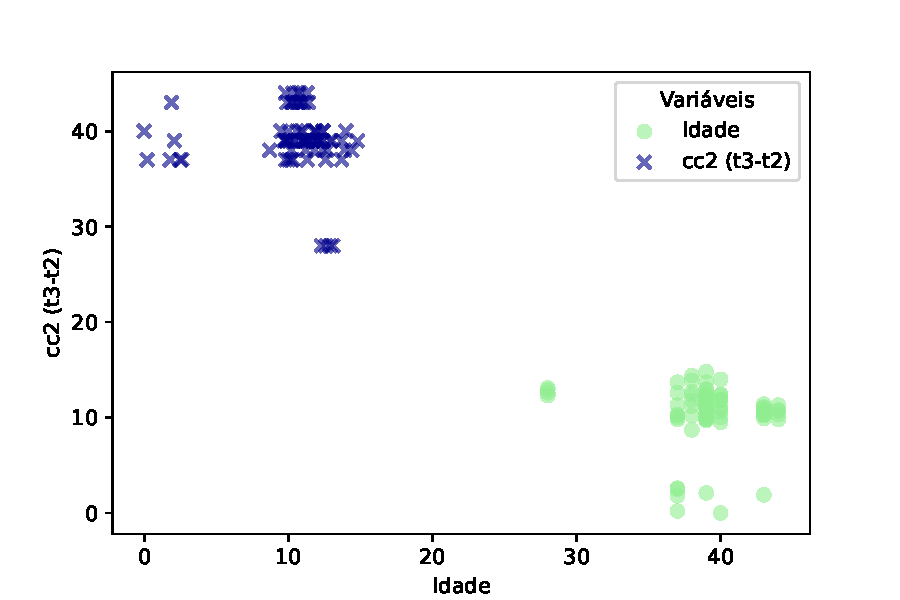
\includegraphics[scale=0.35]{figuras/Spearman/idade-cc2.pdf}
        \vspace{0.3cm}
        \begin{minipage}{\linewidth}
            \centering
            \scriptsize{Fonte: Autoras (2025)}
        \end{minipage}
    \end{minipage}
\end{figure}
\FloatBarrier

\begin{figure}[h]
    \captionsetup{font=footnotesize, justification=centering, labelsep=period, position=above}
    \centering
    \begin{minipage}[b]{0.45\linewidth}
        \caption{Dispersão entre Idade e s2 (t4-t3) Coeficiente de Spearman: -0.24}
        \label{fig:idade-s2}
        \centering
        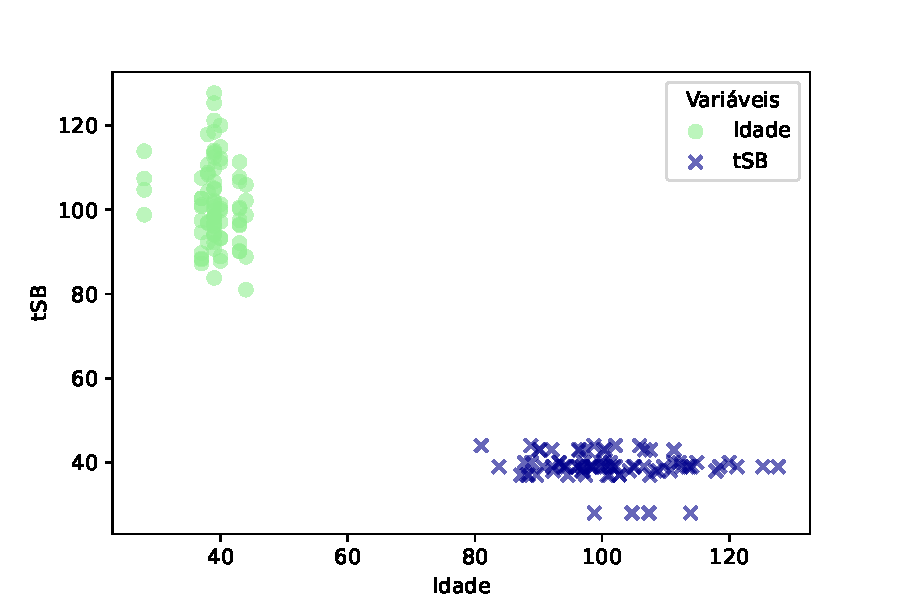
\includegraphics[scale=0.47]{figuras/Spearman/idade-tSB.pdf}
        \vspace{0.3cm}
        \begin{minipage}{\linewidth}
            \centering
            \scriptsize{Fonte: Autoras (2025)}
        \end{minipage}
    \end{minipage}
    \hspace{0.05\linewidth}
    \begin{minipage}[b]{0.45\linewidth}
        \caption{Dispersão entre Idade e s3 (t8-t5) Coeficiente de Spearman: -0.28}
        \label{fig:idade-s3}
        \centering
        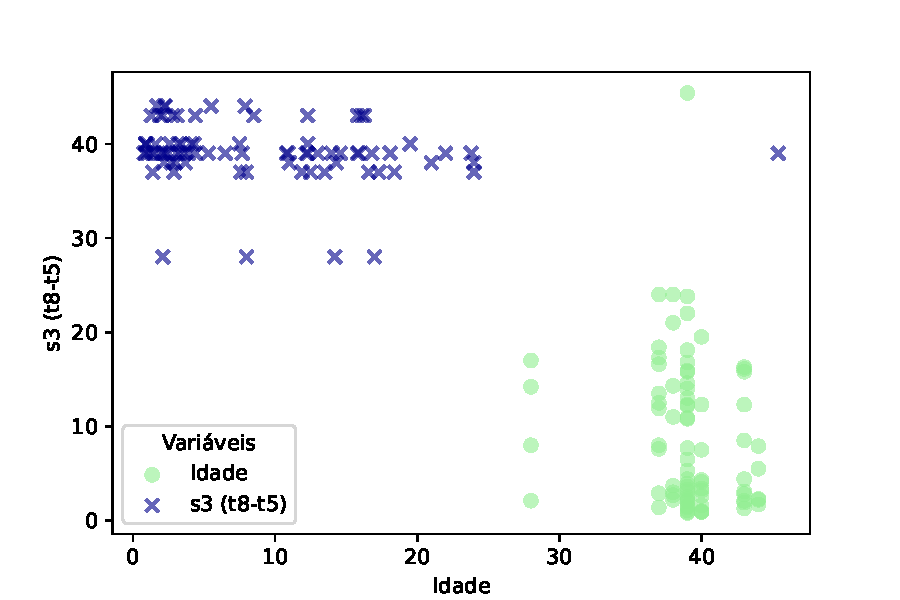
\includegraphics[scale=0.35]{figuras/Spearman/idade-s3.pdf}
        \vspace{0.3cm}
        \begin{minipage}{\linewidth}
            \centering
            \scriptsize{Fonte: Autoras (2025)}
        \end{minipage}
    \end{minipage}
\end{figure}
\FloatBarrier

Analisando os índices positivos, temos \textbf{tB-tSB (0.20)} e \textbf{cc3 (t5-t3) (0.20)} com valores que sugerem que a elevação de uma variável está de forma sutil ligada ao crescimento da outra. Em relação ao intervalo entre o estágio de \textbf{cc3} (Figura \ref{fig:idade-cc3}) e \textbf{tB-tSB} (Figura \ref{fig:idade-tB-tSB}) nos embriões de mulheres mais velhas aumenta levemente. Este crescimento pode sugerir que, mesmo com atrasos em etapas posteriores, o embrião busca se ajustar para compensar o desenvolvimento inicial mais lento.

\begin{figure}[h]
    \captionsetup{font=footnotesize, justification=centering, labelsep=period, position=above}
    \centering
    \begin{minipage}[b]{0.45\linewidth}
        \caption{Dispersão entre Idade e tB-tSB Coeficiente de Spearman: 0.20}
        \label{fig:idade-tB-tSB}
        \centering
        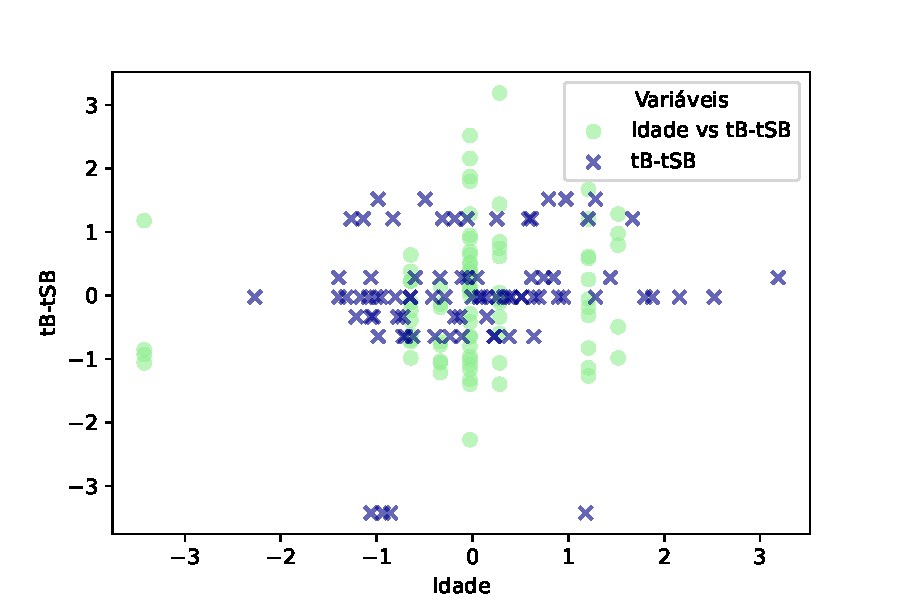
\includegraphics[scale=0.35]{figuras/Spearman/idade-tB-tSB.pdf}
        \vspace{0.3cm}
        \begin{minipage}{\linewidth}
            \centering
            \scriptsize{Fonte: Autoras (2025)}
        \end{minipage}
    \end{minipage}
    \hspace{0.05\linewidth}
    \begin{minipage}[b]{0.45\linewidth}
        \caption{Dispersão entre Idade e cc3 (t5-t3) Coeficiente de Spearman: 0.20}
        \label{fig:idade-cc3}
        \centering
        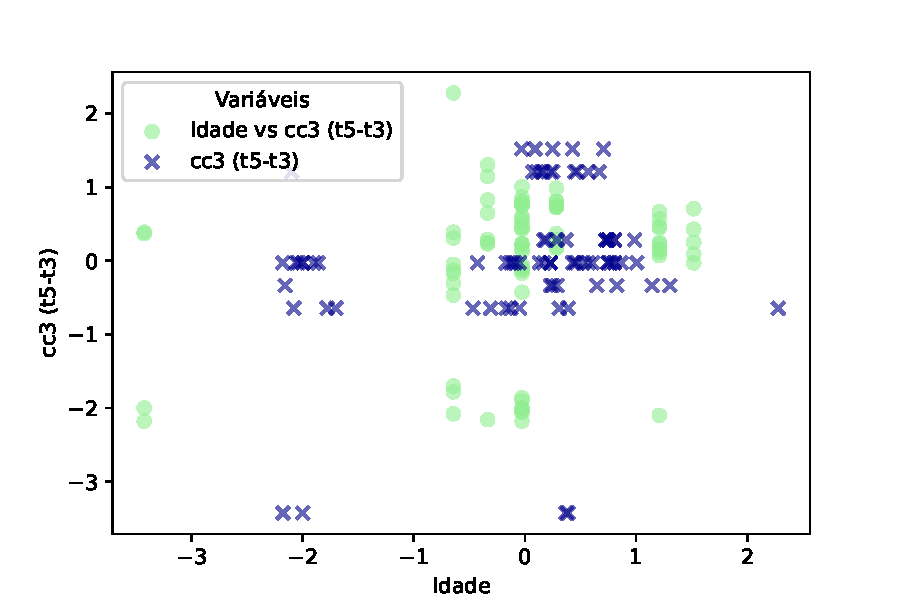
\includegraphics[scale=0.35]{figuras/Spearman/idade-cc3.pdf}
        \vspace{0.3cm}
        \begin{minipage}{\linewidth}
            \centering
            \scriptsize{Fonte: Autoras (2025)}
        \end{minipage}
    \end{minipage}
\end{figure}
\FloatBarrier

E por fim temos a \textbf{Ploidia (-0,50), a correlação negativa mais relevante entre todas as outras variáveis}, que sugere uma relação negativa, demonstrando que a alta idade materna está ligada a uma diminuição na proporção de embriões euploides. Esta informação indica que embriões de mães mais velhas contêm uma proporção reduzida de euploidia, o que pode estar ligado a uma queda na qualidade genética dos embriões. Portanto, a idade materna é um dos elementos chave na diminuição da euploidia embrionária, e conseguimos comprovar esse dado juntamente com as informações que possui na literatura, como citado por \textit{Fertility and Ageing} \cite{eshre2005}, que também reitera que o aumento da aneuploidia em embriões está diretamente associado ao envelhecimento materno.

\subsection*{Idade}
